\section{SELU ByteNet}

The Simplified ByteNet experiments indicates that, the compression and decompression layers are necessary, and the normalization layers are very expensive. From these observations it makes sense to analyse whether the normalization layers are actually necessary for the network to converge.

The experiment in figure \ref{fig:result:selu-bytenet:bytenet-nonorm-wmt} is the ``Memorizing WMT NewsTest'' experiment on the ByteNet model without normalization layers. The experiment ran for 300 epochs.

\begin{figure}[h]
    \centering
    \includegraphics[scale=1]{bytenet-nonorm/validation-memorize-wmt.pdf}
    \caption{Shows BLEU score and cross entropy loss for the German to English WMT NewsTest dataset using the ByteNet model without any normalization layers. The exponential moving average used a forget factor of $0.1$.}
    \label{fig:result:selu-bytenet:bytenet-nonorm-wmt}
\end{figure}

Figure \ref{fig:result:selu-bytenet:bytenet-nonorm-wmt} shows that the non-normalized ByteNet model never completely memorizes the training dataset as it should. It is possible that it could still learn actual translation when trained on the Europarl v7 dataset, however, it is not very likely.

Recently a new paper showed that it is possible to create a ``self-normalizing neural network''. This means that normalization isn't done explicitly by a normalization layer, but instead the network is created such that the parameters will convergence to weights that ensures normalized internal values.

The ``self-normalizing neural network'' was achieved by using a different activation function and weight initialization. Primarily it is the activation function that is responsible for making the network \textit{self-normalizing}, the initialization is primarily just to ensure a reasonable starting point \cite[https://arxiv.org/pdf/1706.02515.pdf]{selu}.

The activation function is a variation on the exponential-linear-unit (ELU), which is similar to the ReLU activation function. The difference is that two constants ($\lambda, alpha$) are added:
\begin{equation}
\mathrm{SELU}(x) = \lambda \begin{cases}
  x & x > 0 \\
  \alpha (\mathrm{exp}(x) - 1) & x \le 0
\end{cases},\quad \text{where: } \begin{array}{c}
  \alpha = 1.6732632423 \\
  \lambda = 1.0507009873
\end{array}
\end{equation}

The initialization should then be done such that $\mathbb{E}[z_{h_\ell}] = 0$ and $\mathrm{var}[z_{h_\ell}] = 1$. This is achieved by initializing the weights such that:
\begin{equation}
\mathrm{Var}[w_{h_{\ell-1}, h_{\ell}}] = \frac{1}{H_{\ell-1}} \quad \Rightarrow \quad r = \sqrt{\frac{3}{H_{\ell-1}}}
\end{equation}
where $r$ is the symmetric uniform distribution parameter, similarly to that used in He-Initialization.

\begin{figure}[h]
    \centering
    \includegraphics[scale=1]{bytenet-selu/validation-memorize-wmt.pdf}
    \caption{Shows BLEU score and cross entropy loss for the German to English WMT NewsTest dataset using the SELU ByteNet. The exponential moving average used a forget factor of $0.1$.}
    \label{fig:result:selu-bytenet:bytenet-selu-wmt}
\end{figure}

\todo[inline]{Await new results.}
\todo[inline]{Synthetic digits shows similar results as the normalized ByteNet model. \ref{appendix:result:bytenet-selu}.}

\clearpage
\subsection{Performance Profiling}

\todo[inline]{Show performance profile of selu-bytenet}

\subsection{WMT Translation Task}
